%!TEX program = xelatex
\documentclass[10pt]{article}
\usepackage{amsthm}
\usepackage{amssymb}
\usepackage{amsmath}
\usepackage{mathrsfs}
\usepackage{titlesec}
\usepackage{xcolor}
\usepackage{enumerate}
\usepackage{bm}
\usepackage{tikz}
\usepackage{listings}
\usetikzlibrary{arrows}
\usepackage{subfigure}
\usepackage{graphicx,booktabs,multirow}
\usepackage[a4paper]{geometry}
\usepackage{upquote}
\usepackage{float}
\usepackage{pdfpages}

\geometry{verbose,tmargin=2cm,bmargin=2cm,lmargin=2cm,rmargin=2cm}
\geometry{verbose,tmargin=2cm,bmargin=2cm,lmargin=2cm,rmargin=2cm}
\lstset{language=Matlab}
\lstset{breaklines}

\input defs.tex

\newtheorem{proposition}{Proposition}
\newtheorem{remark}{Remark}

\titleformat*{\section}{\centering\LARGE\scshape}
\renewcommand{\thesection}{\Roman{section}}
\lstset{language=Matlab,tabsize=4,frame=shadowbox,basicstyle=\footnotesize,
keywordstyle=\color{blue!90}\bfseries,breaklines=true,commentstyle=\color[RGB]{50,50,50},stringstyle=\ttfamily,numbers=left,numberstyle=\tiny,
  numberstyle={\color[RGB]{192,92,92}\tiny},backgroundcolor=\color[RGB]{245,245,244},inputpath=code}

\begin{document}

\date{\today}
\title{Introduction to Machine Learning, Fall 2023 \\
	Homework 2\\
	\small (Due Tuesday Nov. 14 at 11:59pm (CST))}
\maketitle

\begin{enumerate}[1.]


	\item \defpoints{10} [Convex Optimization Basics]
	      \begin{itemize}
		      \item[(a)] Proof any norm $f:\mathbb{R}^{n}\rightarrow\mathbb{R}$ is convex.~\defpoints{2}
		      \item[(b)] Determine the convexity (i.e., convex, concave or neither) of $f(x_1,x_2)=x_1^2/x_2$ on $\mathbb{R}\times\mathbb{R}_{>0}$.~\defpoints{2}
		      \item[(c)] Determine the convexity of $f(x_1,x_2)=x_1/x_2$ on $\mathbb{R}_{>0}^{2}$.~\defpoints{2}
			  \item[(d)] Recall Jensen's inequality $f(\mathbb{E}(X)) \leq \mathbb{E}(f(X))$ if $f$ is convex for any random variable $X$. 
			  Proof the log sum inequality: 
			  \[
				\sum_{i=1}^{n} a_i \log \frac{a_i}{b_i} \geq \left( \sum_{i=1}^{n} a_i\right) \log \frac{\sum_{i=1}^{n} a_i}{\sum_{i=1}^{n} b_i} 
			  \]
			  where $a_1,\ldots,a_n$ and $b_1,\ldots,b_n$ are positive numbers. Hints: $f(x)=x\log x$ is strictly convex.~\defpoints{4}
	      \end{itemize}


		  \textbf{Solution:}
		  \begin{enumerate}[(a)]
			\item
			let $f(x)$ is $p$-norm, so $f(\theta x)=\theta f(x)$, and $f(x+y)\leq f(x)+f(y)$

			then, $\theta f(x_1)+(1-\theta)f(x_2)=f(\theta x_1)+f((1-\theta)x_2)\geq f(\theta x_1+(1-\theta)x_2)$

			so, the norm is convex.
			\item 
			$$\frac{\partial^2 f}{\partial x_1^2}=\frac{2}{x_2}$$
			$$\frac{\partial^2 f}{\partial x_1x_2}=-\frac{2x_1}{x_2^2}$$
			$$\frac{\partial^2 f}{\partial x_2^2}=\frac{2x_1^2}{x_2^3}$$
			$$\nabla^2f=\begin{bmatrix}
				\frac{2}{x_2}&-\frac{2x_1}{x_2^2}\\-\frac{2x_1}{x_2^2}&\frac{2x_1^2}{x_2^3}
			\end{bmatrix}$$
			$$y^T\nabla^2fy=\frac{2y_1^2}{x_2}-\frac{4x_1y_1y_2}{x_2^2}+\frac{2x_1^2y_2^2}{x_2^3}=\frac{2}{x_2^3}(x_2y_1-x_1y_2)^2\geq0$$
			then, it is convex
			\item 
			$$\frac{\partial^2 f}{\partial x_1^2}=0$$
			$$\frac{\partial^2 f}{\partial x_1x_2}=-\frac{1}{x_2^2}$$
			$$\frac{\partial^2 f}{\partial x_2^2}=\frac{2x_1}{x_2^3}$$
			$$\nabla^2f=\begin{bmatrix}
				0&-\frac{1}{x_2^2}\\-\frac{1}{x_2^2}&\frac{2x_1}{x_2^3}
			\end{bmatrix}$$
			$$y^T\nabla^2fy=-\frac{2y_1y_2}{x_2^2}+\frac{2x_1y_2^2}{x_2^3}=\frac{2y_2}{x_2^2}(\frac{x_1y_2}{x_2}-y_1)$$
			$$y^T\nabla^2-fy=\frac{2y_1y_2}{x_2^2}-\frac{2x_1y_2^2}{x_2^3}=\frac{2y_2}{x_2^2}(y_1-\frac{x_1y_2}{x_2})$$
			when $\frac{x_1y_2}{x_2}<y_1$, $y^T\nabla^2fy<0$. So $y^T\nabla^2fy$ is not semipositive definite matrix. then, the function is not convex.
			
			when $\frac{x_1y_2}{x_2}>y_1$, $y^T\nabla^2-fy<0$. So $y^T\nabla^2-fy$ is not semipositive definite matrix. then, the function is not concave.
			\item
			let $x_i=\frac{a_i}{b_i}$, and $P(x=x_i)=\frac{b_1}{\sum_{i=1}^nb_i}$.
			then, $$E(f(x))=\sum_{i=1}^na_i\log\frac{a_i}{b_i},\ \ \ \ \ \ f(E(x))=(\sum_{i=1}^na_i)\log\frac{\sum_{i=1}^na_i}{\sum_{i=1}^nb_i}$$
			and because $f(x)$ is convex function, so $E(f(x))\geq f(E(x))$, then $\sum_{i=1}^{n} a_i \log \frac{a_i}{b_i} \geq \left( \sum_{i=1}^{n} a_i\right) \log \frac{\sum_{i=1}^{n} a_i}{\sum_{i=1}^{n} b_i}$
		  \end{enumerate}

	      \newpage

	\item \defpoints{10} [Linear Methods for Classification] 
	Consider the ``Multi-class Logistic Regression'' algorithm. Given training set 
	$\mathcal{D}=\{(x^i,y^i)\mid i=1,\ldots,n\}$ where $x^i\in \mathbb{R}^{p+1}$ is the 
	feature vector and $y^i\in \mathbb{R}^{k}$ is a one-hot binary vector indicating 
	$k$ classes. We want to find the parameter $\hat{\beta}=[\hat{\beta}_1,\ldots,\hat{\beta}_k]\in \mathbb{R}^{(p+1)\times k}$ 
	that maximize the likelihood for the training set. Introducing the softmax 
	function, we assume our model has the form 
	\[
		p(y_c^i=1\mid x^i;\beta) = \frac{\exp(\beta_c^\top x^i)}{\sum_{c'}\exp(\beta_{c'}^\top x^i)},
	\]
	where $y_c^i$ is the $c$-th element of $y^i$.
		\begin{itemize}
		\item[(a)] Complete the derivation of the conditional log likelihood for our model, which is
		\begin{align*}
			\ell(\beta) = \ln \prod_{i=1}^{n} p(y_t^i\mid x^i;\beta)
			=\sum_{i=1}^{n}\sum_{c=1}^{k}\left[ y_c^i(\beta_c^\top x^i) - y_c^i\ln \left(\sum_{c'}\exp(\beta_{c'}^\top x^i) \right)\right].
		\end{align*}
		For simplicity, we abbreviate $p(y_t^i=1\mid x^i;\beta)$ as $p(y_t^i\mid x^i;\beta)$, where 
		$t$ is the true class for $x^i$.~\defpoints{4}
		\item[(b)] Derive the gradient of $\ell(\beta)$ w.r.t. $\beta_1$, i.e., 
		\[
			\nabla_{\beta_1}\ell(\beta) = \nabla_{\beta_1} \sum_{i=1}^{n}\sum_{c=1}^{k}\left[ y_c^i(\beta_c^\top x^i) - y_c^i\ln \left(\sum_{c'}\exp(\beta_{c'}^\top x^i) \right)\right].
		\]
		Remark: Log likelihood is always concave; thus, we can optimize our model 
		using gradient ascent. (The gradient of $\ell(\beta)$ w.r.t. $\beta_2,\ldots,\beta_k$ is similar, you don't need to write them)~\defpoints{6}
		\end{itemize}
		\textbf{Solution:}
		\begin{enumerate}[(a)]
			\item 
			$$\min\mathbf{KL}(p(y_c^i|x^i,\beta)||p(y_t^i|x^i,\beta))=\int p(y_c^i|x^i,\beta)\log p(y_c^i|x^i,\beta)dx_i-\int p(y_t^i|x^i,\beta)\log p(y_c^i|x^i,\beta)dx_i$$
			$$=C-\int p(y_t^i|x^i,\beta)\log p(y_c^i|x^i,\beta)dx_i=C-\frac{1}{N}\sum_{i=1}^n\log p(y_t^i|x^i,\beta)$$
			$$\Rightarrow \ell(\beta)=\sum_{i=1}^n\log p(y_t^i|x^i,\beta)=\sum_{i=1}^{n}\sum_{c=1}^{k}\left[ y_c^i(\beta_c^\top x^i) - y_c^i\ln \left(\sum_{c'}\exp(\beta_{c'}^\top x^i) \right)\right]$$
			\item 
			$$\nabla_{\beta_1}\ell(\beta) = \nabla_{\beta_1} \sum_{i=1}^{n}\sum_{c=1}^{k}\left[ y_c^i(\beta_c^\top x^i) - y_c^i\ln \left(\sum_{c'}\exp(\beta_{c'}^\top x^i) \right)\right]$$
			$$=\sum_{i=1}^n\left[y^i_1x^i-y^i_1\frac{x^i\exp(\beta_1^Tx^i)}{\sum_{c'}\exp(\beta_{c'}^Tx^i)}\right]=\sum_{i=1}^{n} y_1^i x^i \left[1 - \frac{\exp(\beta_1^\top x^i)}{\sum_{c'}\exp(\beta_{c'}^\top x^i)}\right]$$
		\end{enumerate}
		\newpage

	\item \defpoints{10} [Probability and Estimation]
	Suppose $\mathcal{D}=\{ x_{1}, x_{2}, \ldots, x_{n} \}$ are i.i.d. samples from exponential distribution with parameter 
	$\lambda > 0$, i.e., $X \sim \text{Expo}(\lambda)$. Recall the PDF of exponential distribution is
	\[
		p(x\mid \lambda) = \begin{cases}
		\lambda e^{-\lambda x},&\quad x > 0 \\
		0,&\quad \text{otherwise}
		\end{cases}.
	\]
		\begin{itemize}
		\item[(a)] To derive the posterior distribution of $\lambda$, we assume its prior 
		distribution follows gamma distribution with parameters $\alpha,\beta > 0$, i.e., 
		$\lambda \sim\text{Gamma}(\alpha,\beta)$ (since the range of gamma distribution 
		is also $(0,+\infty)$, thus it's a plausible assumption). The PDF of $\lambda$ is 
		given by
		\[
			p(\lambda\mid \alpha,\beta) = \frac{\beta^{\alpha}}{\Gamma(\alpha)} \lambda^{\alpha-1}e^{-\lambda\beta},
		\]
		where $\Gamma(\alpha) = \int_{0}^{+\infty} t^{\alpha-1}e^{-t}dt,\ \alpha>0$. 
		Show that the posterior distribution $p(\lambda\mid \mathcal{D})$ is also a 
		gamma distribution and identify its parameters. Hints: Feel free to drop 
		constants. \defpoints{4}

		\item[(b)] Derive the maximum a posterior (MAP) estimation for $\lambda$ 
		under $\text{Gamma}(\alpha,\beta)$ prior. \defpoints{3}
		
		\item[(c)] For exponential distribution $\text{Expo}(\lambda)$, $\sum_{i=1}^{n} x_{i}\sim \text{Gamma}(n,\lambda)$ 
		and the inverse sample mean $\frac{n}{\sum_{i=1}^{n} x_{i}}$ is the MLE for $\lambda$. 
		Argue that whether $\frac{n-1}{n}\hat{\lambda}_{MLE}$ is unbiased ($\mathbb{E}(\frac{n-1}{n}\hat{\lambda}_{MLE})=\lambda$). 
		Hints: $\Gamma(z+1)=z\Gamma(z)$, $z > 0$. \defpoints{3}
		\end{itemize}

		
		\textbf{Solution:}
		\begin{enumerate}[(a)]
			\item 
			if all the x is greater than 0:
			$$P(\lambda|\mathcal{D})=\frac{P(\mathcal{D}|\lambda)P(\lambda)}{P(D)}=P(\lambda|\alpha,\beta)\prod_{i=1}^nP(x_i|\lambda)=\frac{\beta^\alpha}{\Gamma(\alpha)}\lambda^{\alpha-1}e^{-\lambda\beta}\prod_{i=1}^{n}(\lambda e^{-\lambda x_i})$$
			$$=\frac{\beta^\alpha}{\Gamma(\alpha)}\lambda^{\alpha+n-1} e^{-\lambda\sum_{i=1}^{n}x_i+\lambda\beta}=\lambda^{\alpha+n-1}e^{-\lambda\sum_{i=1}^nx_i+\lambda\beta}$$
			$$=\frac{(\sum_{i=1}^nx_i+\beta)^{\alpha+n}}{\Gamma(\alpha+n)}\lambda^{\alpha+n-1}e^{-\lambda(\sum_{i=1}^nx_i+\beta)}\sim \mathbf{Gamma}(\alpha+n,\sum_{i=1}^nx_i+\beta)$$
			if there exist one x is not greater than 0, then $P(x|\lambda)=0$, so the posterior $P(\lambda|\mathcal{D})=0$
			\item
			$$\hat\lambda^{\text{MAP}}=\arg\max_{\lambda}P(\lambda|\mathcal{D})$$
			for the Gamma distribution $\mathbf{Gamma}(\alpha,\beta)$, it's PDF is $f(x)=\frac{\beta^\alpha}{\Gamma(\alpha)}x^{\alpha-1}e^{-x\beta}$, the maximum value is at $$\frac{df}{dx}=\frac{\beta^\alpha}{\Gamma(\alpha)}((\alpha-1)x^{\alpha-2}e^{-x\beta}-\beta x^{\alpha-1}e^{-x\beta})=0$$ 
			so its max point is $x=\frac{\alpha-1}{\beta}$ 

			because $\hat\lambda^{\text{MAP}}\sim\mathbf{Gamma}(\alpha+n,\sum_{i=1}^nx_i+\beta)$, so its max point is $\max\hat\lambda^{\text{MAP}}=\frac{\alpha'-1}{\beta'}=\frac{\alpha+n-1}{\sum_{i=1}^nx_i+\beta}$
			$$\Rightarrow\hat\lambda^{\text{MAP}}=\arg\max_{\beta}=\frac{\alpha+n-1}{\sum_{i=1}^{n}x_i+\beta}$$
			\item 
			$$\mathbb{E}(\frac{n-1}{n}\hat\lambda_{\text{MLE}})=\mathbb{E}(\frac{n-1}{\sum_{i=1}^nx_i})=(n-1)\mathbb{E}(\frac{1}{\sum_{i=1}^nx_i})$$
			$$\sum_{i=1}^nx_i\sim\mathbf{Gamma}(n,\lambda)\Rightarrow\mathbb{E}(\frac1{\sum_{i=1}^nx_i})=\int_{0}^{\infty}\frac{1}{x}\cdot\frac{\lambda^n}{\Gamma(n)}x^{n-1}e^{-\lambda x}dx=\frac{\lambda^n}{\Gamma(n)}\int_{0}^{\infty}x^{n-2}e^{-x\lambda}dx$$
			$$=\frac{\lambda}{\Gamma(n)}\int_{0}^{\infty}(\lambda x)^{n-1-1}e^{-\lambda x}d\lambda x=\frac{\lambda}{\Gamma(n)}\Gamma(n-1)=\frac{\lambda}{n-1}$$
			$$\Rightarrow\mathbb{E}(\frac{n-1}{n}\hat\lambda_{\text{MLE}})=\lambda$$
			Therefore, the MLE for $\lambda$ is unbiased.
		\end{enumerate}
		\newpage

	\item \defpoints{10} [Graphical Models]
	Given the following Bayesian Network, 
	\begin{figure}[h]
		\label{fig:bn}
		\vskip 0.2in
		\begin{center}
		\centerline{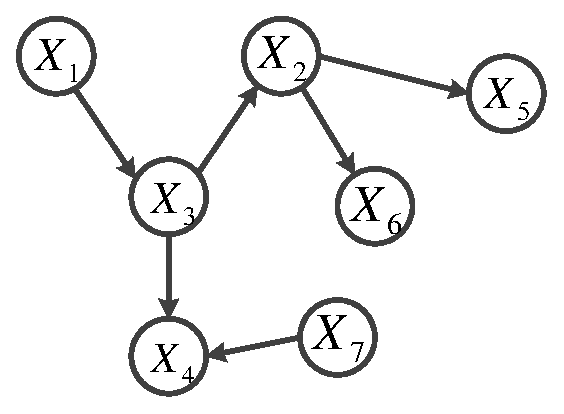
\includegraphics[width=0.4\columnwidth]{figures/bn}}
		%\caption{}
		\end{center}
		\vskip -0.2in
	\end{figure}

	answer the following questions.
		\begin{itemize}
			\item[(a)] Factorize the joint distribution of $X_{1},\cdots,X_{7}$ according 
			to the given Bayesian Network.~\defpoints{2} 
			\item[(b)] Justify whether $X_{1}\perp X_{5}\mid X_{2}$?~\defpoints{2} 
			\item[(c)] Justify whether $X_{5}\perp X_{7}\mid X_{3},X_{4}$?~\defpoints{2} 
			\item[(d)] Justify whether $X_{5}\perp X_{7}\mid X_{4}$?~\defpoints{2} 
			\item[(e)] Write down the variables that are in the Markov blanket of $X_{3}$.~\defpoints{2} 
		\end{itemize}

		\textbf{Solution:}
		\begin{enumerate}[(a)]
			\item 
			$$P(X_1,X_2,X_3,X_4,X_5,X_6,X_7)=P(X_1)P(X_2)P(X_3|X_1)P(X_4|X_3)P(X_5|X_2)P(X_6|X_2)P(X_7)$$
			Note: Different starting points may result in different final answers.
			\item 
			yes. because $X_1$ to $X_5$ is a head-to-tail path. so given $X_2$, $X_1$ and $X_5$ are not connected. so $X_1\perp\!\!\!\perp X_5|X_2$
			\item 
			yes. if given $X_3$, then the path between $X_5$ and $X_7$ must be broken, then they're disconnected. so $X_5\perp\!\!\!\perp X_7|X_3,X_4$
			\item 
			no. because $X_4$ is a head-to-head node, so given $X_4$, the path between $X_5$ and $X_7$ is connected. so $X_5\not\!\perp\!\!\!\perp X_7|X_4$
			\item 
			Markov blanket is containing its co-parent, children and parent. they are $X_1,X_2,X_4,X_7$
		\end{enumerate}

\end{enumerate}

\end{document}